\documentclass[12pt]{article}

\usepackage{amsmath,amsthm,amssymb,amscd,epsfig,url}
\usepackage{fullpage}
\usepackage{times}
\usepackage[T1]{fontenc}
\usepackage[utf8]{inputenc}
\usepackage{fancyvrb}
\usepackage{mathdots}
\newtheorem{theorem}{Theorem}[section]
\newtheorem{lemma}[theorem]{Lemma}
\newtheorem{proposition}[theorem]{Proposition}
\newtheorem{corollary}[theorem]{Corollary}
\newtheorem{conjecture}[theorem]{Conjecture}
\newtheorem{definition}[theorem]{Definition}
\newtheorem{example}[theorem]{Example}
\newtheorem{remark}[theorem]{Remark}

\usepackage{xcolor}
\usepackage{tikz}
\usetikzlibrary{arrows.meta, automata, positioning}

\def\ZZ{{\mathbb Z}}
\def\QQ{{\mathbb Q}}
\def\RR{{\mathbb R}}
\def\TT{{\mathcal{C} T}}
\def\KK{{\mathcal{C} K}}
\newcommand{\hus}{\hfill\break}
\newcommand{\bull}{\textbullet\;\;}
\def\iso{{\operatorname{\ \approx \ }}}   % isomorphism
\def\im{{\operatorname{im}}}              % image
\def\Hom{{\operatorname{Hom}}}           % homomorphisms
\def\line{{\operatorname{line} \,}}       % line graph
\def\sd{{\operatorname{sd \,}}}           % first edge subdivision graph
\def\coker{{\operatorname{coker}}}        % cokernel
\def\lcm{{\operatorname{lcm}}}             % least common multiple
\newcommand{\gcdd}{\gamma}              
\def\del{{\partial}}                      % signed incidence matrix
\def\<{{\langle}} \def\>{{\rangle}}       % Inner product
\def\ZC{{Z^\#}}                           % cycle space
\setlength{\textheight}{9in}               
%\setlength{\textwidth}{6in}               % width of text
%\setlength{\oddsidemargin}{0in}           % odd page left margin
%\setlength{\evensidemargin}{0in}          % even page left margin 

\title{Problem Set 5}
\author{CMSC 27200: Theory of Algorithms}
\date{Assigned February 18, 2026, Due February 24, 2026}

\begin{document}
\maketitle

\thispagestyle{empty}
\section*{Problem 0: Collaborators and Outside Sources}
Who did you collaborate with?
Did you use any outside sources?
\section*{Problem 1: Ford-Fulkerson (25 points)}
Graph:

    \begin{center}
    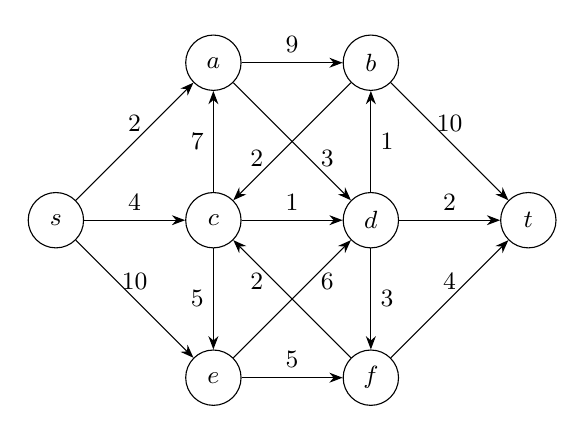
\begin{tikzpicture}[
      mycircle/.style={
         circle,
         draw=black,
         fill=white,
         fill opacity = 0.3,
         text opacity=1,
         inner sep=0pt,
         minimum size=20pt,
         font=\small},
      myarrow/.style={-Stealth},
      node distance=0.6cm and 1.2cm
      ]
      \node[mycircle]  at (-3, 0) (s) {$s$};
      \node[mycircle]  at (-1, 2) (a) {$a$};
      \node[mycircle]  at (1, 2) (b) {$b$};
      \node[mycircle]  at (-1, 0) (c) {$c$};
      \node[mycircle]  at (1, 0) (d) {$d$};
      \node[mycircle]  at (-1, -2) (e) {$e$};
      \node[mycircle]  at (1, -2) (f) {$f$};
      \node[mycircle]  at (3, 0) (t) {$t$};

    \foreach \i/\j/\txt/\p/\pp in {% start node/end node/text/position
      s.45/a.225/2/above/0.5,
      s.00/c.180/4/above/0.5,
      s.315/e.135/10/above/0.5,
      a.00/b.180/9/above/0.5,
      a.315/d.135/3/above/0.8,
      b.225/c.45/2/above/0.8,
      b.315/t.135/10/above/0.5,
      c.90/a.270/7/left/0.5,
      c.00/d.180/1/above/0.5,
      c.270/e.90/5/left/0.5,
      d.90/b.270/1/right/0.5,
      d.270/f.90/3/right/0.5,
      d.00/t.180/2/above/0.5,
      e.45/d.225/6/below/0.8,
      e.00/f.180/5/above/0.5,
      f.135/c.315/2/below/0.8,
      f.45/t.225/4/above/0.5
      }
       \draw [myarrow] (\i) -- node[font=\small,\p,pos=\pp] {\txt} (\j);


    \end{tikzpicture}
    \end{center}
\noindent Current flow:
    \begin{center}
    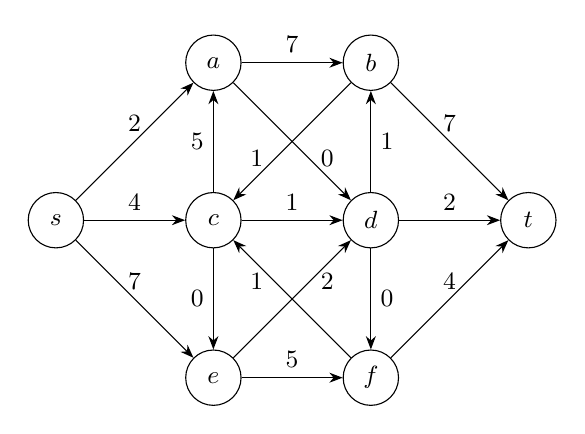
\begin{tikzpicture}[
      mycircle/.style={
         circle,
         draw=black,
         fill=white,
         fill opacity = 0.3,
         text opacity=1,
         inner sep=0pt,
         minimum size=20pt,
         font=\small},
      myarrow/.style={-Stealth},
      node distance=0.6cm and 1.2cm
      ]
      \node[mycircle]  at (-3, 0) (s) {$s$};
      \node[mycircle]  at (-1, 2) (a) {$a$};
      \node[mycircle]  at (1, 2) (b) {$b$};
      \node[mycircle]  at (-1, 0) (c) {$c$};
      \node[mycircle]  at (1, 0) (d) {$d$};
      \node[mycircle]  at (-1, -2) (e) {$e$};
      \node[mycircle]  at (1, -2) (f) {$f$};
      \node[mycircle]  at (3, 0) (t) {$t$};

    \foreach \i/\j/\txt/\p/\pp in {% start node/end node/text/position
      s.45/a.225/2/above/0.5,
      s.00/c.180/4/above/0.5,
      s.315/e.135/7/above/0.5,
      a.00/b.180/7/above/0.5,
      a.315/d.135/0/above/0.8,
      b.225/c.45/1/above/0.8,
      b.315/t.135/7/above/0.5,
      c.90/a.270/5/left/0.5,
      c.00/d.180/1/above/0.5,
      c.270/e.90/0/left/0.5,
      d.90/b.270/1/right/0.5,
      d.270/f.90/0/right/0.5,
      d.00/t.180/2/above/0.5,
      e.45/d.225/2/below/0.8,
      e.00/f.180/5/above/0.5,
      f.135/c.315/1/below/0.8,
      f.45/t.225/4/above/0.5
      }
       \draw [myarrow] (\i) -- node[font=\small,\p,pos=\pp] {\txt} (\j);


    \end{tikzpicture}
    \end{center}
Starting from the given flow, implement the Ford-Fulkerson algorithm by hand to find a maximum flow from $s$ to $t$ and find a minimum cut proving that this flow is a maximum flow. For each iteration (including the iteration where the algorithm terminates), show the residual graph and the flow path that you find from $s$ to $t$ (if such a path exists).
\section*{Problem 2: Ford-Fulkerson With No Backwards Edges (20 points)}
What happens if we don't have backwards edges in the Ford-
Fulkerson algorithm? In other words, what happens if, after an iteration of Ford-Fulkerson where we find a path from $s$ to $t$ and route $c_{min}$ flow through it
(where $c_{min}$ is the minimum remaining capacity of an edge on this path), we
just reduce the capacities of the edges along this route by $c_e$ in the residual
graph (and don't increase the capacities of the edges going backwards by $c_{min}$
as we are ignoring them)?

Your friend conjectures that the Ford-Fulkerson algorithm with no backwards edges
will still always give a constant factor approximation, i.e., there exists a
constant $c > 0$ such that if the maximum flow is $F$, regardless of how we choose
the paths from $s$ to $t$ we will obtain a total flow of at least $cF$ from $s$ to
$t$. Is your friend's conjecture correct? Either prove your friend's conjecture or
describe how to construct a counterexample for any $c > 0$.\\
\\
Hint is available.

\section*{Problem 3: Store Supplier (25 points)}
You are a supplier which supplies $m$ different products to $n$ stores. You have the following constraints:
\begin{enumerate}
\item For each product $i \in [m]$, you have a supply $s_i$ of product $i$.
\item For each product $i \in [m]$ and each store $j \in [n]$, store $j$ wants a maximum of $c_{ij}$ of product $i$.
\item Each store $j \in [n]$ will buy a maximum of $b_j$ products in total.
\end{enumerate}
What is the maximum total number of products $T$ that you can sell to these stores and which products should you sell to each store in order to achieve this? In other words, can you find $\{x_{ij}: i \in [m], j \in [n]\}$ such that 
\begin{enumerate}
\item For all $i \in [m]$, $\sum_{j=1}^{n}{x_{ij}} \leq s_i$.
\item For all $i \in [m]$ and $j \in [n]$, $x_{ij} \leq c_{ij}$.
\item For all $j \in [n]$, $\sum_{i=1}^{m}{x_{ij}} \leq b_j$.
\end{enumerate}
and your total sales $T = \sum_{i=1}^{m}{\sum_{j=1}^{n}{x_{ij}}}$ is maximized?

Letting $S = \sum_{i=1}^{m}{s_i}$, give an algorithm for this problem whose runtime is polynomial in $S$, $m$, and $n$. Prove that your algorithm is correct and analyze its runtime. \\
\\
Hint is available.
\vspace{5mm}
\newpage
\section*{Problem 4: Carpooling (30 points)}
A group of $k$ people $p_1,\ldots,p_k$ are carpooling to work for $n$ days and they need to choose drivers for each day. However, only a subset of the people go to work each day. Also, they would like to divide up the driving duties fairly. In particular, no person should drive more than the expected number of times they would drive if the driver was chosen randomly each day (rounded up).
\begin{example}
Let's say there are 3 people $p_1,p_2,p_3$ carpooling for 4 days and the people carpooling on each day are as follows:
\begin{enumerate}
\item On day $1$, all $3$ people are carpooling.
\item On day $2$, $p_1$ and $p_3$ are carpooling.
\item On day $3$, $p_2$ and $p_3$, are carpooling.
\item On day $4$, $p_2$ and $p_3$ are carpooling again.
\end{enumerate}
In this case, if the driver was chosen randomly each day, the expected number of times $p_1$ drives is $\frac{1}{3} + \frac{1}{2} = \frac{5}{6}$. The expected number of times $p_2$ drives is $\frac{1}{3} + 2\cdot\frac{1}{2} = \frac{4}{3}$. The expected number of times $p_3$ drives is $\frac{1}{3} + 3\cdot\frac{1}{2} = \frac{11}{6}$. Thus, we can have $p_1$ drive at most $1$ time and we can have $p_2$ and $p_3$ drive at most $2$ times. One way to do this is to have $p_1$ drive on day $2$, have $p_2$ drive on day $3$, and have $p_3$ drive on days $1$ and $4$
\end{example}
We can state this problem more precisely as follows. We are given subsets the subsets of people $\{S_j\}$ who are carpooling each day and we want to choose drivers $\{p_{i_j}\}$ such that 
\begin{enumerate}
\item $\forall j \in [n] (i_j \in S_j)$ (the driver for each day is one of the people carpooling for that day)
\item $\forall i \in [k]\left(|\{j: i_j = i\}| \leq \lceil\sum_{j \in [n]:i \in S_j}{\frac{1}{|S_j|}}\rceil\right)$ (no person drives more than the expected number of times they should drive rounded up)
\end{enumerate}

Show that such a driving schedule always exists, give an algorithm to find such a driving schedule, prove that your algorithm is correct, and analyze its runtime. The runtime of your algorithm should be polynomial in $k$ and $n$.\\
\\
Hint is available.

\newpage
\noindent Hints:\\
\\
2. What happens if your path from $s$ to $t$ goes back and forth across the minimum
cut? Alternatively, can you construct an example where many possible paths from $s$
to $t$ are blocked by taking a single path?\\
\\
3. You should reduce this problem to max flow. To prove that your algorithm is correct, you should do two things:
\begin{enumerate}
\item Show that if there is a sales plan with total sales $T$ then there is a flow with value $T$.
\item Show that given an integer-valued flow with value $T$, you can extract a sales plan with total sales $T$.
\end{enumerate}
Note that you can and should use Ford-Fulkerson as a black box so you do not need to justify why Ford-Fulkerson works.\\
\\
4. Express this problem as a max flow problem with vertices corresponding to the people and vertices corresponding to the days. Can you construct a maximum flow (not necessarily an integer-valued flow) for this problem without running Ford-Fulkerson? Given this, what happens if you run Ford-Fulkerson on this problem?

For proving that your algorithm is correct, you can use Ford-Fulkerson as a black box so you just need to prove that you can extract a valid schedule from the flow given by Ford-Fulkerson.


\newpage
\section*{Conversion Note}
This file uses the provided starter TeX for the original problem statements and TikZ graph relationships, then includes the full solution text extracted from the matching PDF. The graph drawings do not need to be pixel-identical to the PDF; the directed edges and weights are preserved in the starter TeX where provided.

\newpage
\section*{Full Solution Text Extracted from PDF}
\begin{Verbatim}[breaklines=true,fontsize=\small]
                                     Problem Set 5
                          CMSC 27200: Theory of Algorithms
                 Assigned February 18, 2026, Due February 24, 2026


Problem 0: Collaborators and Outside Sources
Who did you collaborate with? Did you use any outside sources?


Problem 1: Ford-Fulkerson (25 points)
Graph:
                                                     9
                                             a               b
                                    2                                10
                                         7       2       3       1
                                    4                1               2
                              s              c               d            t
                                    10           2       6           4
                                         5                       3
                                                     5
                                             e               f

Current flow:
                                                     7
                                             a               b
                                    2                                7
                                         5       1       0       1
                                    4                1               2
                              s              c               d            t
                                    7            1       2           4
                                         0                       0
                                                     5
                                             e               f

    Starting from the given flow, implement the Ford-Fulkerson algorithm by hand to find a maxi-
mum flow from s to t and find a minimum cut proving that this flow is a maximum flow. For each
iteration (including the iteration where the algorithm terminates), show the residual graph and the
flow path that you find from s to t (if such a path exists).

--- page break ---
Solution
Residual graph of the given flow:

                                                         2
                                             a                   b
                                                         7
                                                     3
                             2                                               3
                                         5 2                     1
                                                 1                   7
                                                     1
                     s           4           c                           2
                                                         1       d               t
                                                     1       2
                                     3
                                         5                       3
                             7                                           4
                                                     4       1
                                             e                   f
                                                         5

   There is an s-t path s -> e -> d -> c -> b -> t that we can use to push one unit of flow. The
new residual graph will be the following:

                                                         2
                                             a                   b
                                                         7
                                                     3
                             2                                               2
                                         5 2                     1
                                                 2                   8


                     s           4           c                           2
                                                         1       d               t
                                                     1       3
                                     2
                                         5                       3
                             8                                           4
                                                     3       1
                                             e                   f
                                                         5




                                                         2

--- page break ---
                                                                   1
                                                   a                               b
                                                                   8
                                                               3
                               2                                                                   1
                                               6 1                                 1
                                                           2                               9


                       s           4               c                                           2
                                                                   1               d                   t
                                                               2       4
                                       1
                                               5                               1 2
                               9                                                                   4
                                                               2
                                                   e                               f
                                                                   5

    Now there is no more s-t path in the residual graph and the following flow is a max-flow, the
value of this flow is 15:

                                                                   8
                                                           a               b
                                           2                                           9
                                                       6       0       0       1
                                           4                       0                   2
                                   s                       c               d                   t
                                           9                   2       4               4
                                                       0                       1
                                                                   5
                                                           e               f


    To find a min-cut with capacity equal to the value of this flow, let S be the set of vertices
that are reachable from s in the final residual graph: S = {s, d, e, f }. Let T = V \ S. We
claim that the capacity of (S, T ) is equal to 15. Indeed, the edges pointing from S to T include
(s, a), (s, c), (d, b), (d, t), (f, c), (f, t). The sum of the capacities is 2 + 4 + 1 + 2 + 2 + 4 = 15.


Problem 2: Ford-Fulkerson With No Backwards Edges (20 points)
What happens if we don't have backwards edges in the Ford-Fulkerson algorithm? In other words,
what happens if, after an iteration of Ford-Fulkerson where we find a path from s to t and route
cmin flow through it (where cmin is the minimum remaining capacity of an edge on this path),
we just reduce the capacities of the edges along this route by ce in the residual graph (and don't
increase the capacities of the edges going backwards by cmin as we are ignoring them)?
    Your friend conjectures that the Ford-Fulkerson algorithm with no backwards edges will still
always give a constant factor approximation, i.e., there exists a constant c > 0 such that if the
maximum flow is F , regardless of how we choose the paths from s to t we will obtain a total flow
of at least cF from s to t. Is your friend's conjecture correct? Either prove your friend's conjecture

                                                                   3

--- page break ---
or describe how to construct a counterexample for any c > 0.

Hint is available.

Solution
The conjecture is false. For any c > 0, a counterexample can be constructed as follows. Let
m = ?1/c? + 1, and let G = (V, E) where

                                V = {s, t, x1 , . . . , xm , y1 , . . . , ym }

and

E = {(s, xi ) : 1 <= i <= m}?{(xi , yi ) : 1 <= i <= m}?{(yi , t) : 1 <= i <= m}?{(yi , xi+1 ) : 1 <= i <= m-1}.

Each edge in E has capacity 1. The following is an example when m = 3:

                                             x1              y1




                               s             x2              y2                  t




                                             x3              y3


      The maximum flow of this graph is m (using m vertex-disjoint paths s -> xi -> yi -> t).
However, if Ford-Fulkerson without backwards edges takes the path s -> x1 -> y1 -> x2 -> y2 ->
? ? ? -> xm -> ym -> t first, this saturates all edges (xi , yi ), leaving no further augmenting paths.
This gives a total flow of only 1.
      Since m > 1/c, we have 1/m < c, so the ratio of the flow obtained to the maximum flow is
1/m < c. Since c > 0 was arbitrary, the conjecture is false for any constant c > 0.


Problem 3: Store Supplier (25 points)
You are a supplier which supplies m different products to n stores. You have the following con-
straints:

   1. For each product i ? [m], you have a supply si of product i.

   2. For each product i ? [m] and each store j ? [n], store j wants a maximum of cij of product
      i.

   3. Each store j ? [n] will buy a maximum of bj products in total.


                                                      4

--- page break ---
What is the maximum total number of products T that you can sell to these stores and which
products should you sell to each store in order to achieve this? In other words, can you find
{xij : i ? [m], j ? [n]} such that

   1. For all i ? [m], nj=1 xij <= si .
                       P

   2. For all i ? [m] and j ? [n], xij <= cij .

   3. For all j ? [n], m
                      P
                        i=1 xij <= bj .
                         Pm Pn
                 PmT = i=1 j=1 xij is maximized?
and your total sales
    Letting S = i=1 si , give an algorithm for this problem whose runtime is polynomial in S, m,
and n. Prove that your algorithm is correct and analyze its runtime.

Hint is available.

Solution
Construct the following network G:

    o Create a source vertex s and a sink vertex t. For each i ? [m], create a vertex pi and add an
      edge (s, pi ) with capacity si . For each j ? [n], create a vertex qj and an edge (qj , t) with
      capacity bj .

    o For each i ? [m] and each j ? [n], add an edge (pi , qj ) with capacity cij .

Then we run Ford-Fulkerson on G. Let F be the resulting max-flow. Let xij = f (pi , qj ) for all
i ? [m] and j ? [n]. Return {xij }.
    Correctness: We show that there is an assignment {xij } that achieves a total sales of T if and
only if there exists a flow f with value T and f (pi , qj ) = xij for all i ? [m], j ? [n].
    (=>) Let {xij } be a solution to the problem that achieves total sales T . We define         Pna flow with
value T in G  Pas follows. For all i ? [m] and j ? [n], let f (pi , qj ) = xij , f (s, pi ) = j=1 xij , and
f (qj , t) = m    i=1 xij . Conservation of flow is obvious by construction. Constraints 1 to 3 imply
the flows on edges (s, pi ), (pi , qj ), and (qjP
                                                , t) respectively do PmnotPexceed the capacities. Thus f is
indeed a flow. The value of f is precisely m       i=1 f (s, p i ) =  i=1
                                                                             n
                                                                             j=1 xij = T .
    (<=) Let f be a flow on network      Pm G.PnIf v(f ) = T , we     Pmclaim that {f (pi , qj )} is a solution
that achieves total sales T . Since i=1 j=1 f (pi , qj ) = i=1 f (s, pi ) = T , it remains to check
that {f (pi , qj )} satisfies constraints 1 to 3. For the first constraint, we have si >= f (s, pi ) =
P  n
   j=1 f (pi , qj ) since si is the capacity of the edge (s, pi ) and conservation of flow at pi implies
the equality. The second constraint follows since cij is the capacity of the edge (pi , qj ). The third
                     Pm the capacity of the edge (qj , t) implies bj >= f (qj , t), and by conservation of
constraint is similar:
flow, f (qj , t) = i=1 f (pi , qj ).
    Efficiency: The graph G has m + n + 2 vertices and m + n + mn edges. Constructing it takes
O(mn) time. The max-flow in G has value at most S since the cut ({s}, V \ {s}) has capacity S.
Running Ford-Fulkerson on G takes O(Smn) time, which dominates the time for constructing G.
Thus the total running time is O(Smn).


                                                      5

--- page break ---
Problem 4: Carpooling (30 points)
A group of k people p1 , . . . , pk are carpooling to work for n days and they need to choose drivers
for each day. However, only a subset of the people go to work each day. Also, they would like
to divide up the driving duties fairly. In particular, no person should drive more than the expected
number of times they would drive if the driver was chosen randomly each day (rounded up).

Example 0.1. Let's say there are 3 people p1 , p2 , p3 carpooling for 4 days and the people carpool-
ing on each day are as follows:

   1. On day 1, all 3 people are carpooling.

   2. On day 2, p1 and p3 are carpooling.

   3. On day 3, p2 and p3 , are carpooling.

   4. On day 4, p2 and p3 are carpooling again.

In this case, if the driver was chosen randomly each day, the expected number of times p1 drives is
1
3
  + 12 = 56 . The expected number of times p2 drives is 13 + 2 ? 12 = 43 . The expected number of times
p3 drives is 13 + 3 ? 12 = 11
                            6
                              . Thus, we can have p1 drive at most 1 time and we can have p2 and p3
drive at most 2 times. One way to do this is to have p1 drive on day 2, have p2 drive on day 3, and
have p3 drive on days 1 and 4

    We can state this problem more precisely as follows. We are given subsets the subsets of people
{Sj } who are carpooling each day and we want to choose drivers {pij } such that

   1. ?j ? [n](ij ? Sj ) (the driver for each day is one of the people carpooling for that day)
                                                   
                                                1
                                   P
   2. ?i ? [k] |{j : ij = i}| <= ? j?[n]:i?Sj |Sj | ? (no person drives more than the expected num-
      ber of times they should drive rounded up)

    Show that such a driving schedule always exists, give an algorithm to find such a driving sched-
ule, prove that your algorithm is correct, and analyze its runtime. The runtime of your algorithm
should be polynomial in k and n.

Hint is available.

Solution
Construct the following network G:

    o Create a source vertex s and a sink vertex t. For each day j ? [n], create a vertex dj and an
                      Pcapacity 1. For each driver i ? [k], create a vertex pi and an edge (pi , t)
      edge (s, dj ) with
      with capacity ? j?[n]:i?Sj |S1j | ?.

    o For each j ? [n] and for each driver i who goes to work on day j, add an edge (dj , pi ). Set
      the capacity of the edge to be 1.

                                                  6

--- page break ---
Then run Ford-Fulkerson on G. Let f be the resulting max-flow. We pick driver i on day j iff
f (dj , pi ) = 1.
     Correctness: First we show that the max-flow value of G is n. It suffices to construct a flow
with value n since the cut ({s}, V \ {s}) has      P capacity n.     For j ? [n], i ? [k], let f (s, dj ) = 1,
                 1                                             1
f (dj , pi ) = |Sj | for i ? Sj , and f (pi , t) = j?[n]:i?Sj |Sj | . By construction, conservation of flow
is satisfied and the value of this flow is nj=1 f (s, dj ) = n. It remains to check that the flow on
                                                 P

each edge is at most the capacity. Indeed, f (dj , pi ) = |S1j | <= 1 and f (pi , t) <= ? j?[n]:i?Sj |S1j | ?, as
                                                                                        P

desired.
     Now, since the capacities are integers, Ford-Fulkerson will find an integral max-flow. Since the
edges (dj , pi ) have capacity 1, the flow on (dj , pi ) is either 0 or 1. Since the capacity of the edge
(s, dj ) is 1, by conservation of flow, for each j there is exactly one i such that f (dj , pi ) = 1 and
hence for each day we pick exactly one driver. By construction of G, driver i works on day j only
if i ? Sj , so the firstPconstraint 1is satisfied. And again, by conservation of flow, each driver i can
be picked at most ? j?[n]:i?Sj |Sj | ? many times, so the second constraint is also satisfied.
     Efficiency: The graph G has k + n + 2 vertices and at most n + k + nk edges. It takes O(kn)
time to construct. Since the max-flow value of G is precisely n, Ford-Fulkerson takes O(kn2 ) time,
which dominates the time for constructing G. Thus, the total running time is O(kn2 ).




                                                      7

--- page break ---
Hints:

2. What happens if your path from s to t goes back and forth across the minimum cut? Alter-
natively, can you construct an example where many possible paths from s to t are blocked by
taking a single path?

3. You should reduce this problem to max flow. To prove that your algorithm is correct, you
should do two things:

  1. Show that if there is a sales plan with total sales T then there is a flow with value T .

  2. Show that given an integer-valued flow with value T , you can extract a sales plan with total
     sales T .

Note that you can and should use Ford-Fulkerson as a black box so you do not need to justify why
Ford-Fulkerson works.

4. Express this problem as a max flow problem with vertices corresponding to the people and
vertices corresponding to the days. Can you construct a maximum flow (not necessarily an integer-
valued flow) for this problem without running Ford-Fulkerson? Given this, what happens if you
run Ford-Fulkerson on this problem?
    For proving that your algorithm is correct, you can use Ford-Fulkerson as a black box so you
just need to prove that you can extract a valid schedule from the flow given by Ford-Fulkerson.




                                                 8

--- page break ---
\end{Verbatim}

\end{document}
